\documentclass{report}
% PACKAGES
\usepackage[utf 8]{inputenc }
\usepackage {mathtools} % math and figures
\usepackage {float} % places figure at point with [H]
\usepackage {filecontents}
\usepackage [numbered,framed]{matlab-prettifier}
% these packages include more math symbols you might use
\usepackage { amsmath , amsfonts , amsthm , amssymb }
% PROJECT Specific Information to Fill Out
\newcommand{\LectureTitle}{Forecasting Financial Market}
\newcommand{\LectureDate }{\today }
\newcommand{\LectureClassName }{ECON 623}
\newcommand{\LatexerName }{Zixin Huang}
\author {Zixin Huang }

% CONFIGURATIONS to make the report look better
\usepackage { setspace }
\usepackage { Tabbing }
\usepackage { fancyhdr }
\usepackage { lastpage }
\usepackage { extramarks }
\usepackage { afterpage }
\usepackage { abstract }
% In case you need to adjust margins :
\topmargin = -0.45 in
\evensidemargin =0 in
\oddsidemargin =0 in
\textwidth =6.5 in
\textheight =9.0 in
\headsep =0.25 in
% Setup the header and footer
\pagestyle{fancy}
\lhead{\LatexerName }
\chead{\LectureClassName : \LectureTitle }
\rhead{\LectureDate }
%\lfoot{\astxmark }
%\cfoot{}
%\rfoot{ Page \ \ thepage \ of \ \ pageref { LastPage }}
\renewcommand\headrulewidth {0.4 pt }
\renewcommand\footrulewidth {0.4 pt }


\usepackage{xcolor,soul}
\sethlcolor{lightgray}
\usepackage{pdfpages}

\usepackage{indentfirst}
\title {\LectureTitle : Homework 2}

\begin{document}
	
\maketitle

\section*{Exercise 1}

\subsection*{Question A}
Function \hl{\textbf{LBtest.m}}:
\lstinputlisting[style = Matlab-editor]{functions/LBtest.m}



\subsection*{Question B}
Function \hl{\textbf{robustLBtest.m}}:
\lstinputlisting[style = Matlab-editor]{functions/robustLBtest.m}



\subsection*{Question C}
\subsubsection*{USD/EUR Exchange Rate}
\begin{figure}[H]
	\centering
	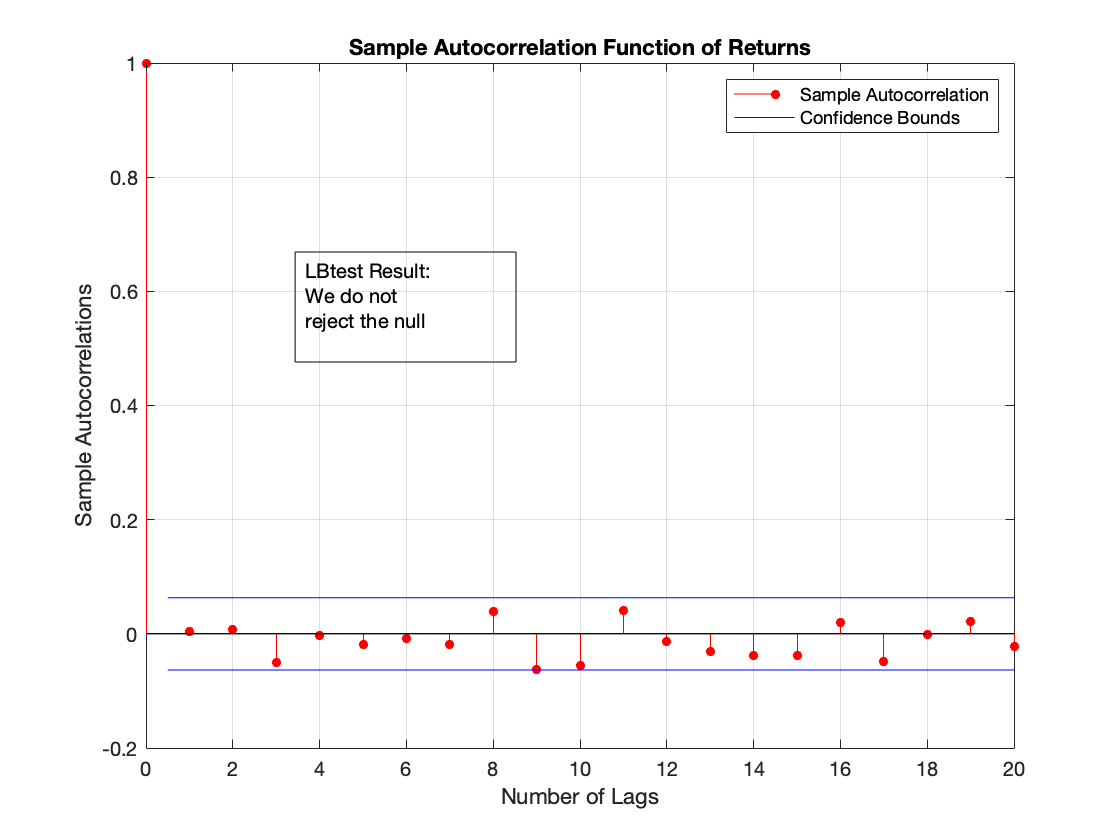
\includegraphics[width = 11cm]{fig/1c11}
	\caption{Sample Autocorrelation Function of Returns} 
\end{figure}


\begin{figure}[H]
	\centering
	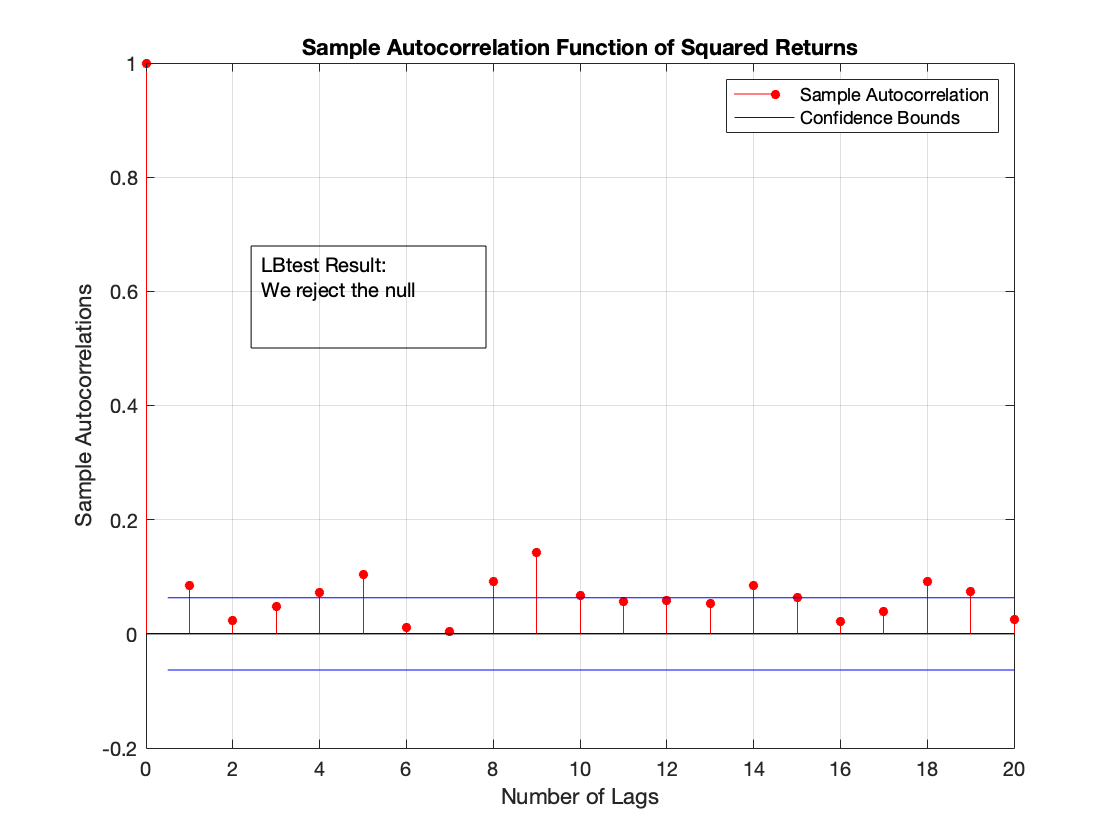
\includegraphics[width = 11cm]{fig/1c12}
	\caption{Sample Autocorrelation Function of Squared Returns} 
\end{figure}





\subsubsection*{SP500}

\begin{figure}[H]
	\centering
	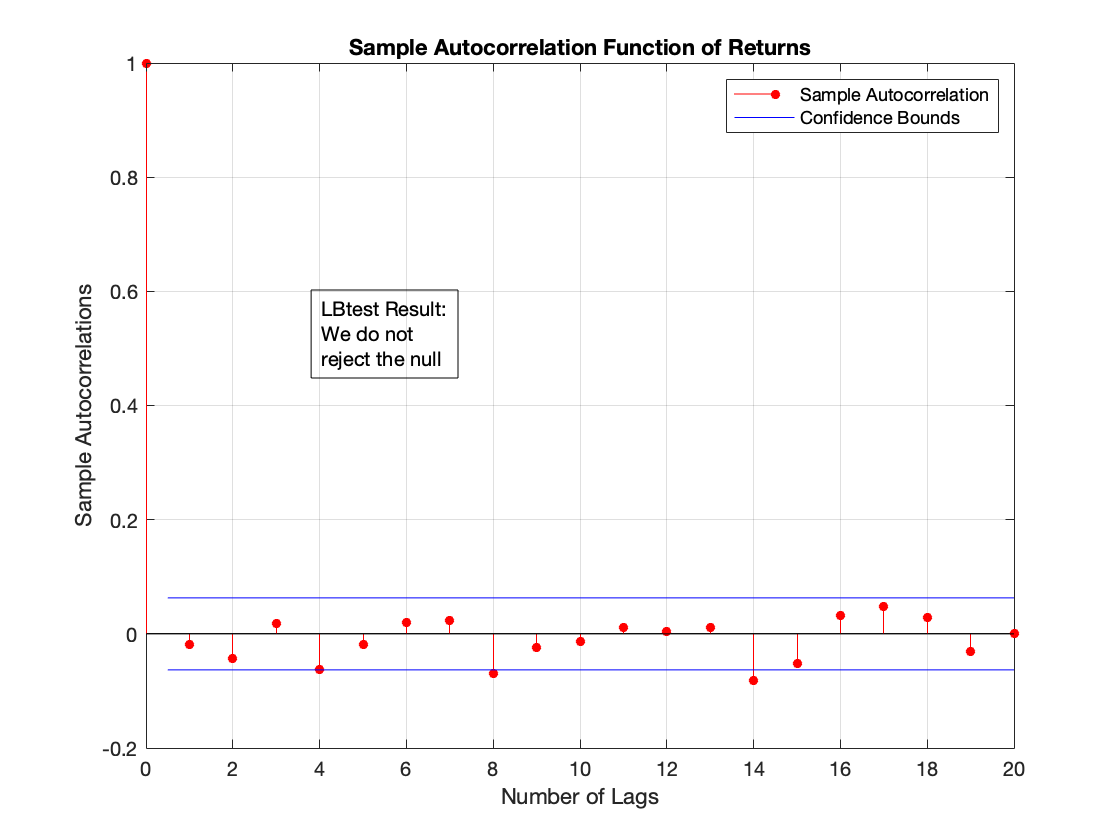
\includegraphics[width = 11cm]{fig/1c21}
	\caption{Sample Autocorrelation Function of Returns} 
\end{figure}


\begin{figure}[H]
	\centering
	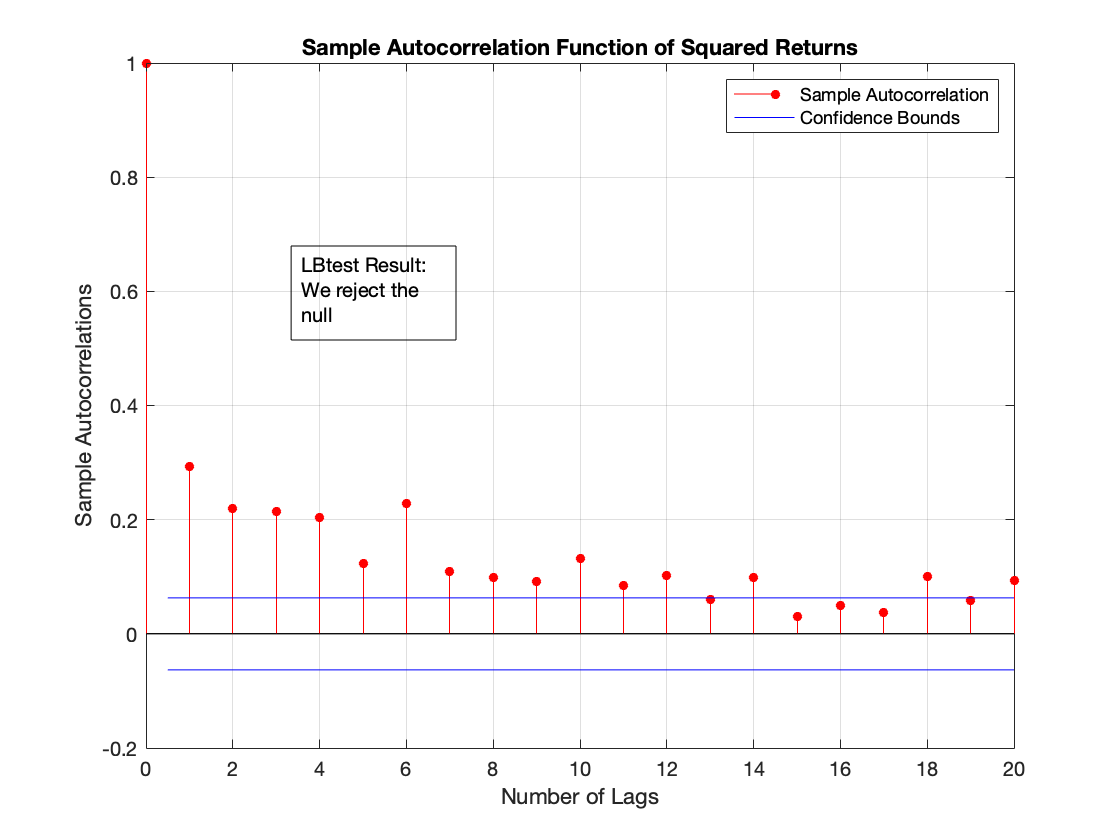
\includegraphics[width = 11cm]{fig/1c22}
	\caption{Sample Autocorrelation Function of Squared Returns} 
\end{figure}




\subsubsection*{NASDAQ100}

\begin{figure}[H]
	\centering
	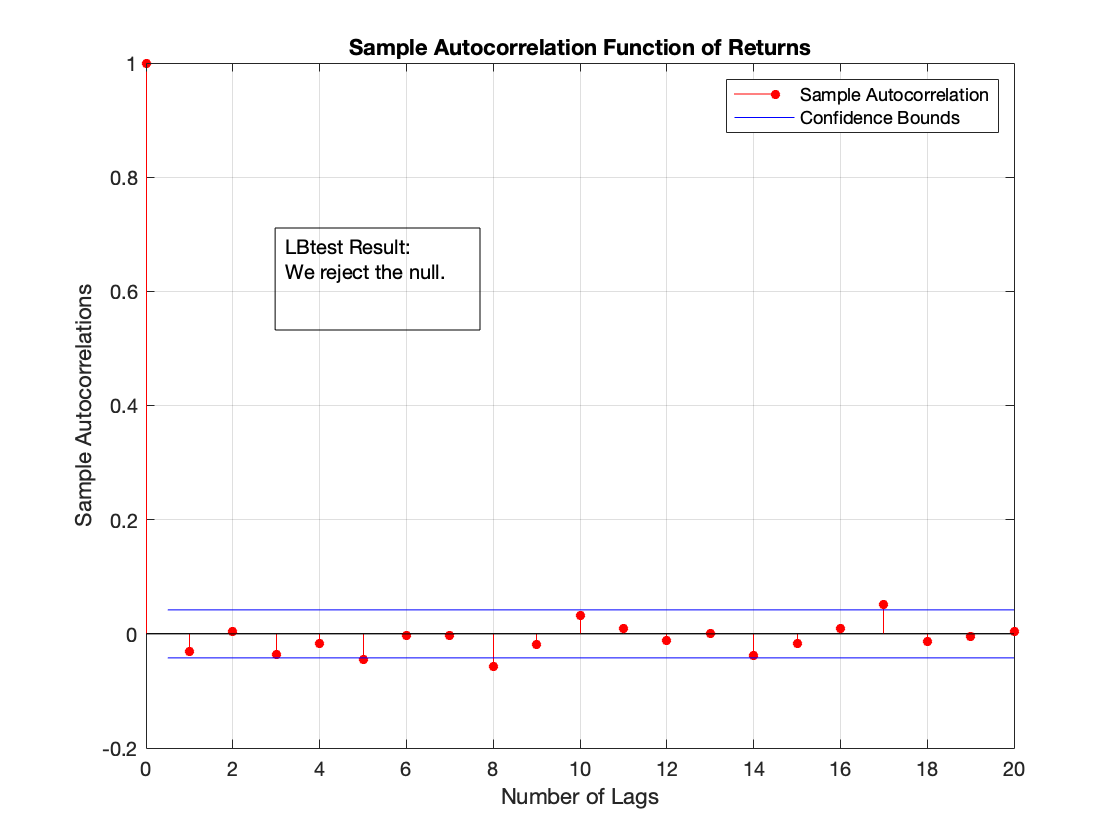
\includegraphics[width = 11cm]{fig/1c31}
	\caption{Sample Autocorrelation Function of Returns} 
\end{figure}


\begin{figure}[H]
	\centering
	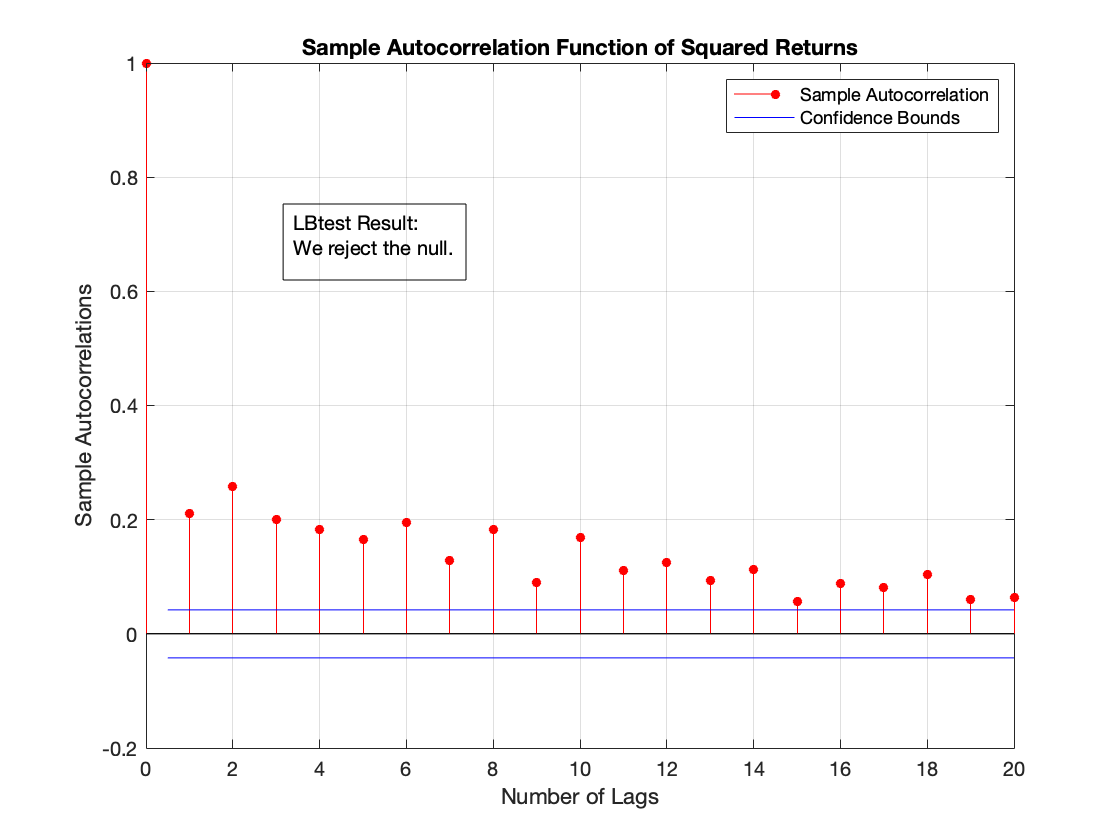
\includegraphics[width = 11cm]{fig/1c32}
	\caption{Sample Autocorrelation Function of Squared Returns} 
\end{figure}




\section*{Exercise 2}

\subsection*{Question A}
Function \hl{\textbf{x3.m}}:
\lstinputlisting[style = Matlab-editor]{functions/x3.m}



\subsection*{Question B}

\begin{table}[H]
	\begin{center}
		\caption{Result of Minimizing $f(x)=|x|^3$}
		\label{tab:table1}
		\vspace{2mm}
		\begin{tabular}{c|c|c|c} 
						
			\textbf{Function} & \textbf{Initial Value}& \textbf{Solution} & \textbf{Function Value}\\
			\hline
			
			\text{fminunc} &  $2$ & 	$0.002$ & 	$8.3202\times 10^{-9}$
	\end{tabular}
	\end{center}
\end{table}

MATLAB process:

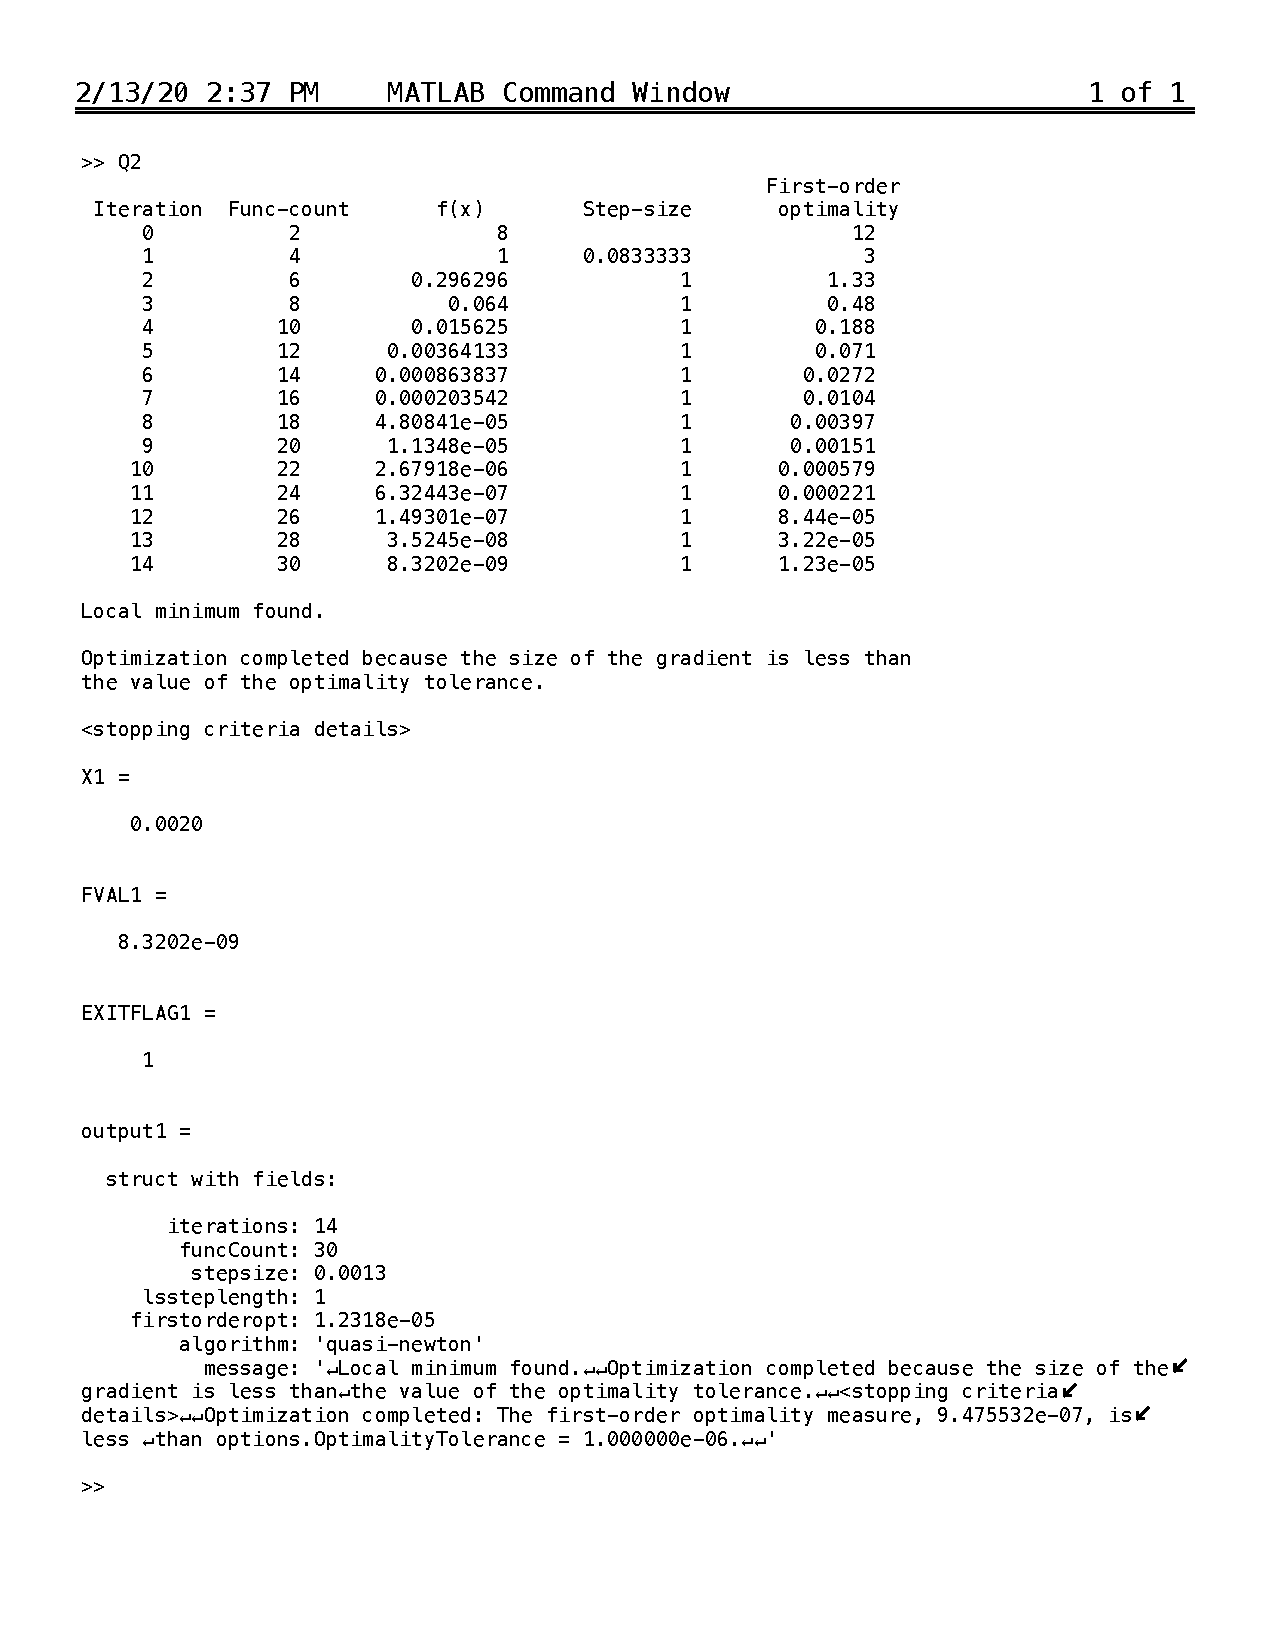
\includepdf[pages=-,pagecommand={},width=\textwidth]{fig/2b.pdf}


\subsection*{Question C}

\begin{table}[H]
	\begin{center}
		\caption{Result of Minimizing $f(x)=|x|^3$}
		\label{tab:table2}
		\vspace{2mm}
		\begin{tabular}{c|c|c|c|c} 
			
			\textbf{Function} & \textbf{Constraints}& \textbf{Initial Value}& \textbf{Solution} & \textbf{Function Value}\\
			\hline
			
			\text{fmincon} &$x\geq 1$ & $3$ & 	$1$ & 	$1$
		\end{tabular}
	\end{center}
\end{table}

MATLAB process:

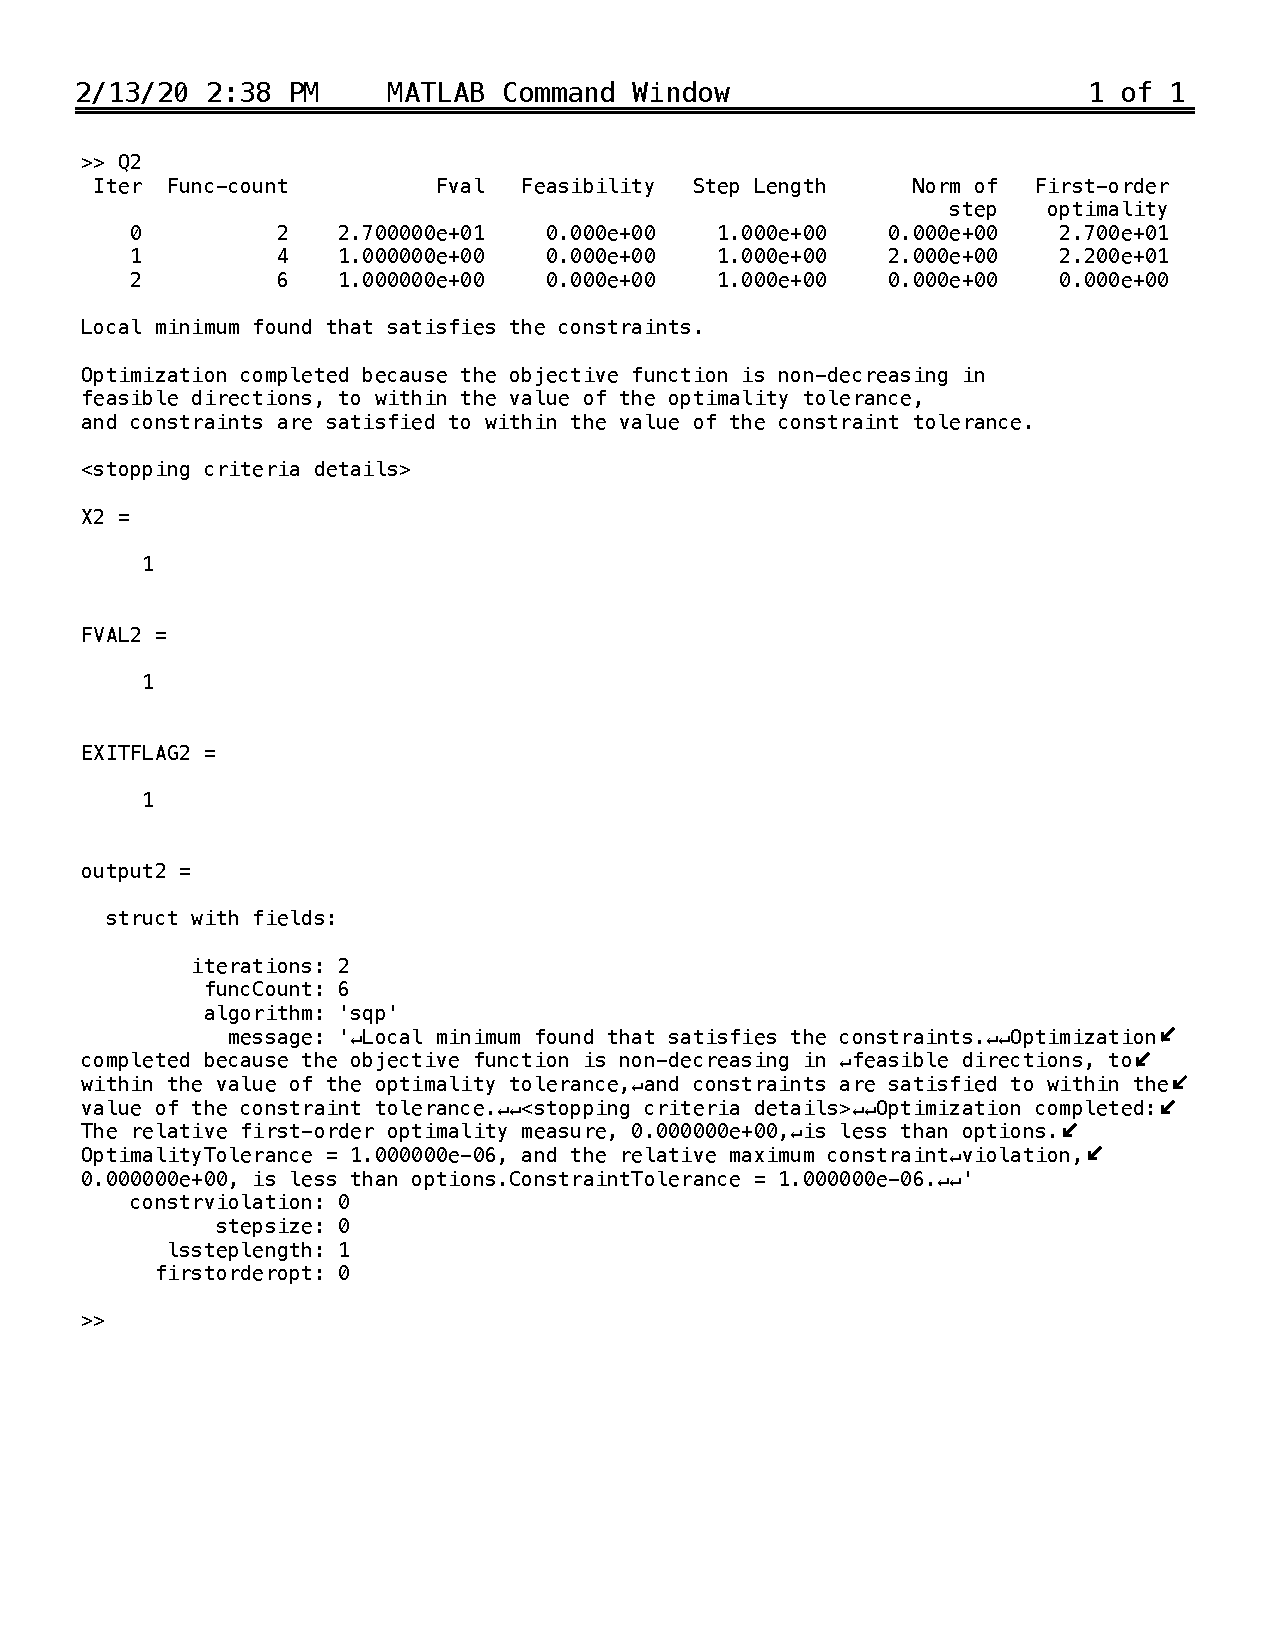
\includepdf[pages=-,pagecommand={},width=\textwidth]{fig/2c.pdf}


\subsection*{Question D}
Function \hl{\textbf{x4.m}}:
\lstinputlisting[style = Matlab-editor]{functions/x4.m}


\subsection*{Question E}
\begin{table}[H]
	\begin{center}
		\caption{Result of Minimizing $f(x)=2(2-x^2)^2+x$}
		\label{tab:table3}
		\vspace{2mm}
		\begin{tabular}{c|c|c|c} 
			
			\textbf{Function} & \textbf{Initial Value}& \textbf{Solution} & \textbf{Function Value}\\
			\hline
			
			\text{fminunc} &  $0$ & 	$-1.4445$ & 	$-1.4295$
		\end{tabular}
	\end{center}
\end{table}



\subsection*{Question F}

\begin{table}[H]
	\begin{center}
		\caption{Result of Minimizing $f(x)=2(2-x^2)^2+x$}
		\label{tab:table4}
		\vspace{2mm}
		\begin{tabular}{c|c|c|c} 
			
			\textbf{Function} & \textbf{Initial Value}& \textbf{Solution} & \textbf{Function Value}\\
			\hline
			
			\text{fminunc} &  $1$ & 	$1.3819$ & 	$1.3982$
		\end{tabular}
	\end{center}
\end{table}

\subsection*{Question G}

\begin{figure}[H]
	\centering
	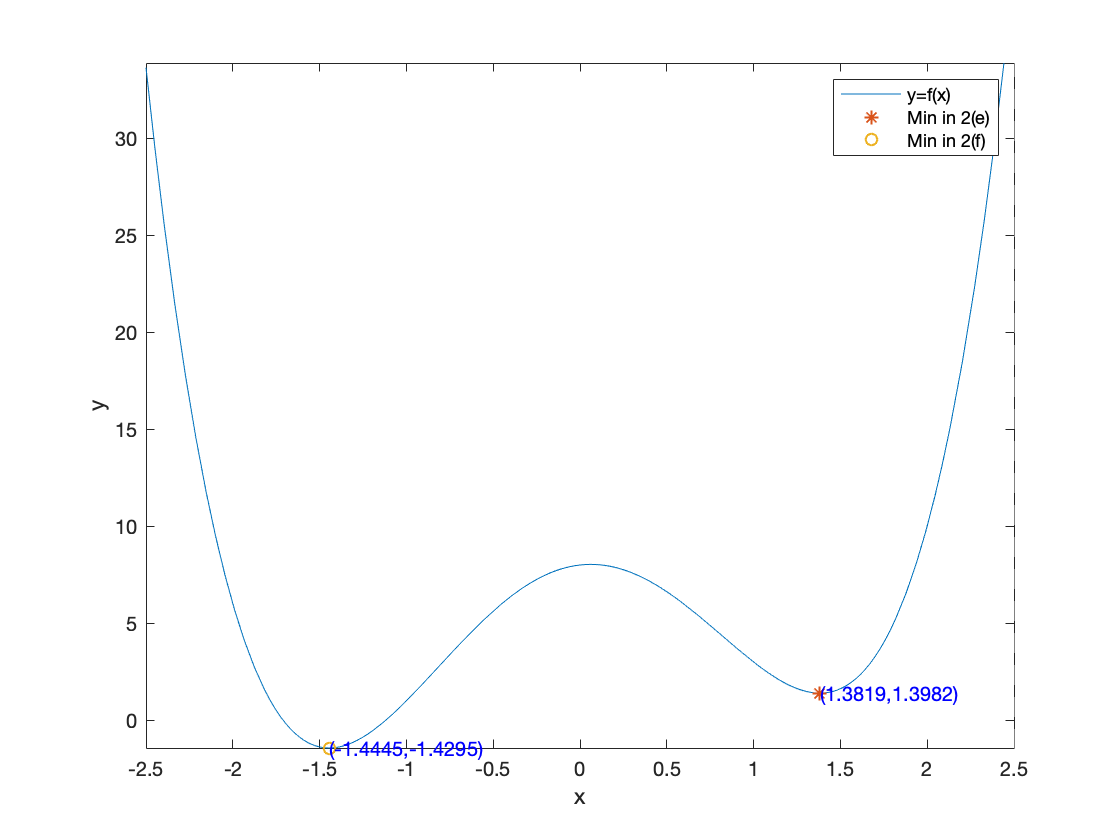
\includegraphics[width = 11cm]{fig/2g}
	\caption{Plot of $f(x)=2(2-x^2)^2+x$ on $[-2.5,2.5]$  } 
\end{figure}




\section*{Exercise 3}
\subsection*{Question A}
Function \hl{\textbf{LL\_normal.m}}:
\lstinputlisting[style = Matlab-editor]{functions/LL_normal.m}


\subsection*{Question B}
In this question, I use the SP500 daily returns from 2015 to 2019 as my time series data.


\begin{table}[H]
	\begin{center}
		\caption{Sample Statistics}
		\label{tab:table5}
		\vspace{2mm}
		\begin{tabular}{c|c|c} 
			
			\textbf{Data}&\textbf{Sample Mean} & \textbf{Sample Variance}\\
			\hline
			
			\text{SP500 Daily Return} &  $2.7163\times 10^{-4}$ & 	$7.5238\times 10^{-5}$
		\end{tabular}
	\end{center}
\end{table}

\begin{table}[H]
	\begin{center}
		\caption{Result of Finding the optimal value of $\hat{\theta}=(\mu, \sigma^2)$}
		\label{tab:table6}
		\vspace{2mm}
		\begin{tabular}{c|c|c|c} 
			
			\textbf{Function} & \textbf{Constraints}& \textbf{Initial Value}& \textbf{Solution} \\
			\hline
			
			\text{fmincon} &$\sigma^2 > 0$ & $(0,1)$ & 	$(2.7166\times 10^{-4}, 7.5156\times 10^{-5})$ 
		\end{tabular}
	\end{center}
\end{table}


From Table 5 and Table 6 we can see that the optimal $\hat{\theta}=(\mu, \sigma^2)$ is nearly identical to the sample mean and the sample variance.\\

MATLAB process:

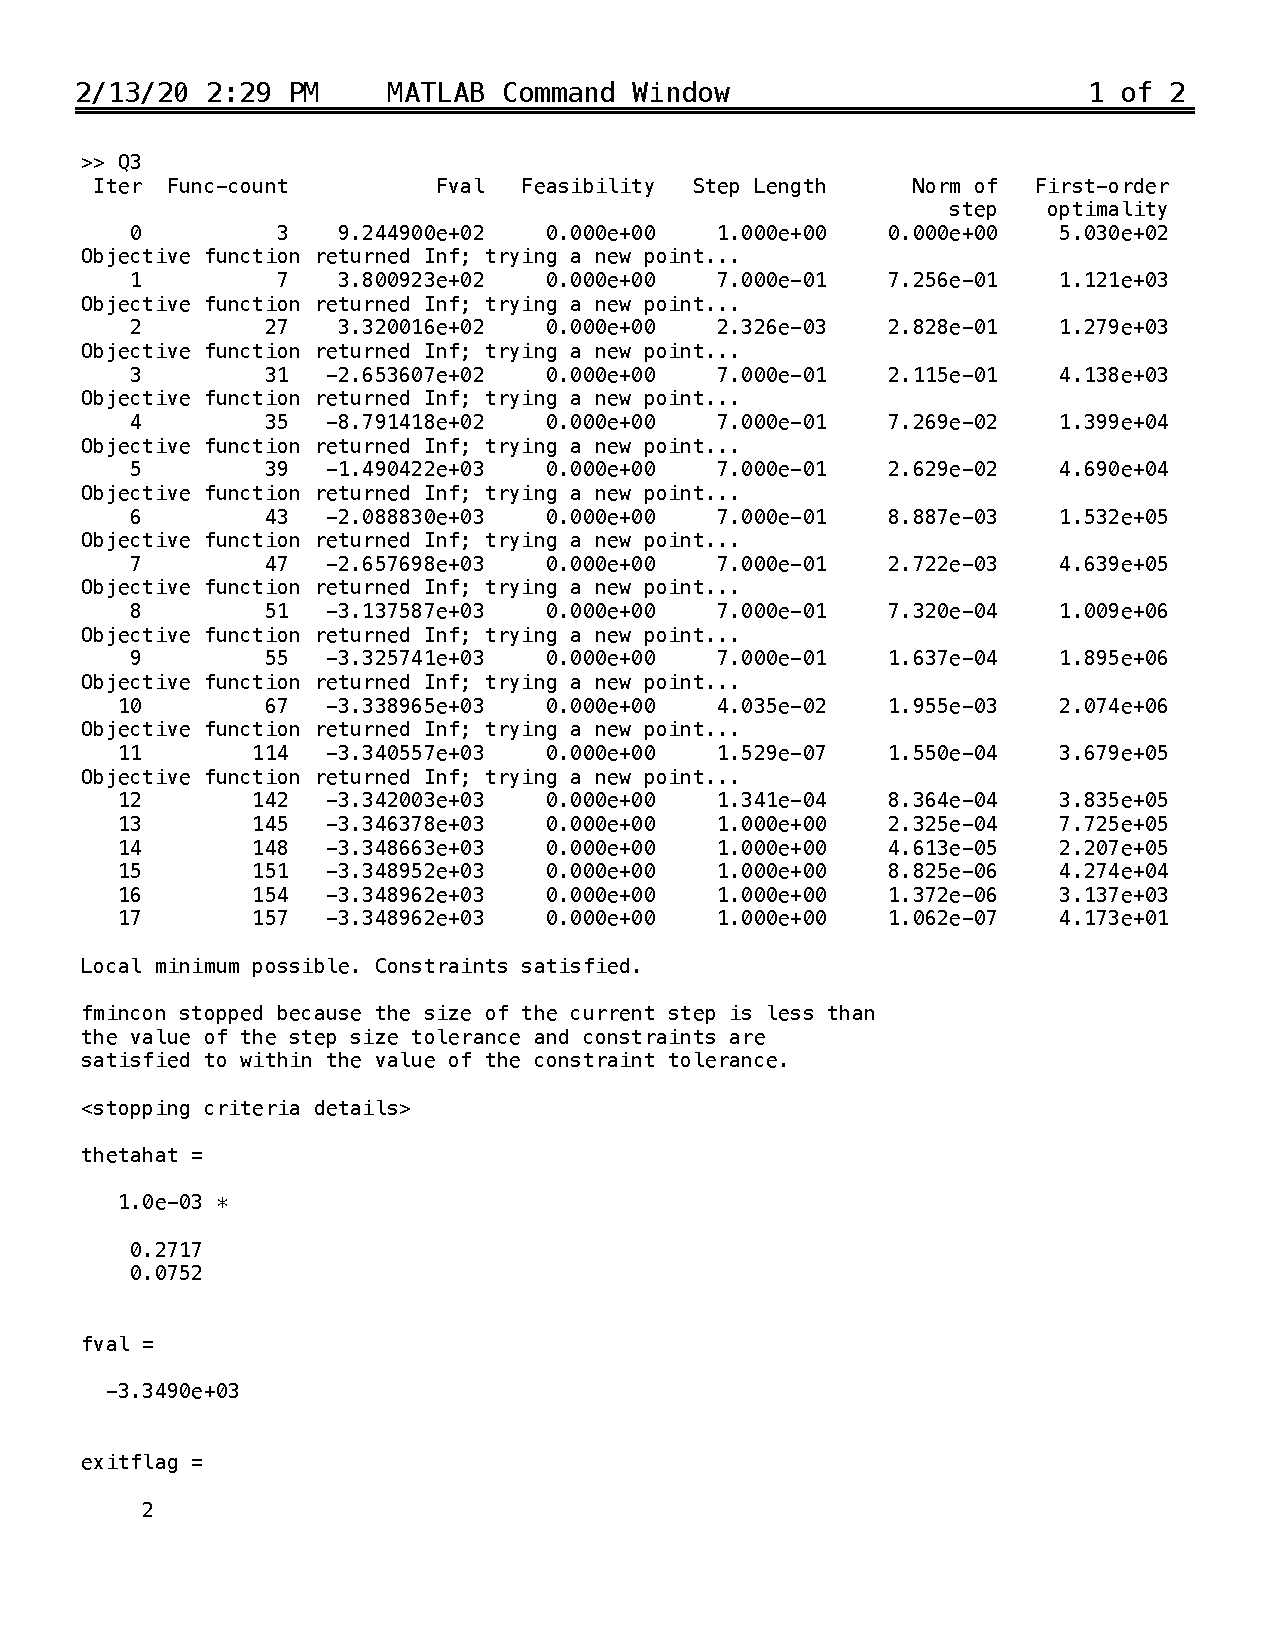
\includepdf[pages=-,pagecommand={},width=\textwidth]{fig/3b.pdf}





\section*{Exercise 4}
In this question, I use the de-meaned daily return of the USD/EUR exchange rates from 2015 to 2019 as my time series data. I choose parameters $\hat{\theta}$ by maximizing the log-likelihood of my data. \\

In GARCH model, we estimate series of variance by:
\begin{equation}
	\sigma_t^2=\omega+\beta \sigma^2_{t-1}+\alpha \epsilon_{t-1}^2
\end{equation}

By applying maximum likelihood, we can find the optimal $\hat{\theta}=(\omega, \beta,\alpha)$:

\begin{table}[H]
	\begin{center}
		\caption{Result of Optimal $\hat{\theta}$}
		\label{tab:table7}
		\vspace{2mm}
		\begin{tabular}{c|c|c} 
			
			\textbf{$\omega$} & \textbf{$\beta$}& \textbf{$\alpha$} \\
			\hline
			
			$1.04\times 10^{-14}$ &$2.4793\times 10^{-8}$ & $0.9997$  
		\end{tabular}
	\end{center}
\end{table}

Then I use the optimal $\hat{\theta}$ I found to generate the GARCH variance series $\sigma_t^2$.

\begin{figure}[H]
	\centering
	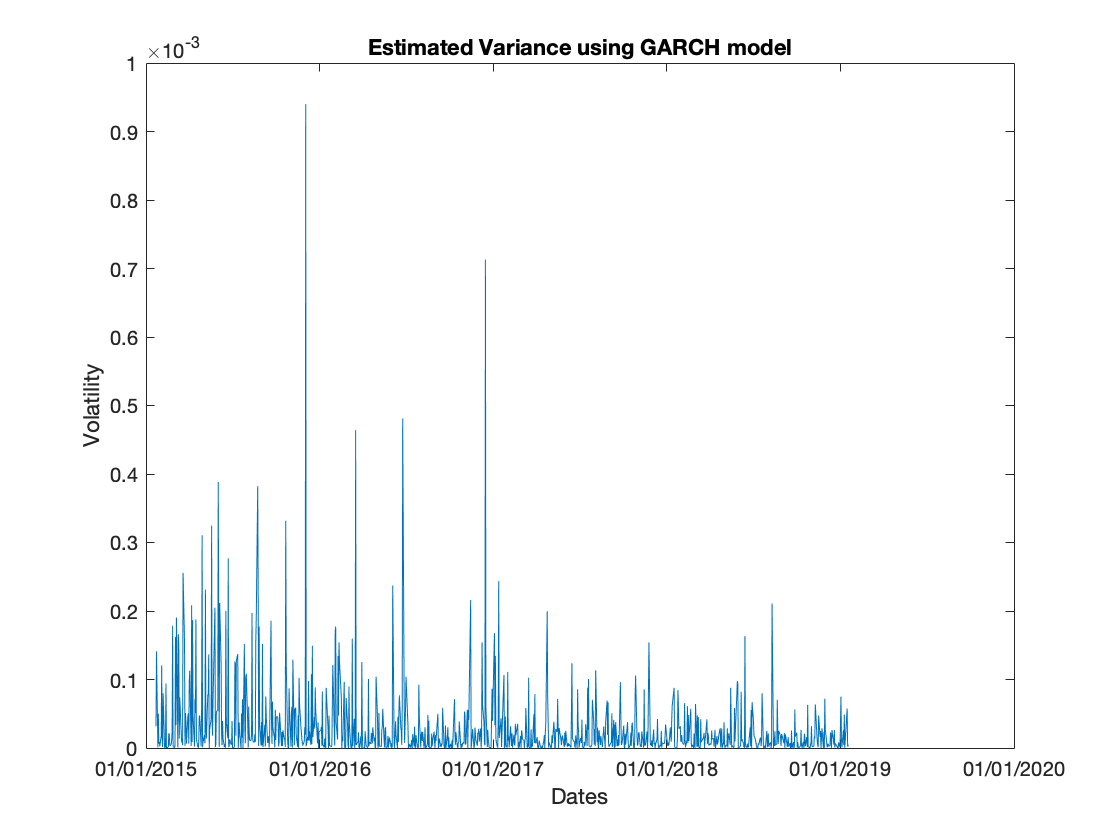
\includegraphics[width = 11cm]{fig/4}
	\caption{GARCH Variance Series of the USD/EUR Exchange Returns } 
\end{figure}






Function \hl{\textbf{garch\_variance.m}}:
\lstinputlisting[style = Matlab-editor]{functions/garch_variance.m}



I compute the log-likelihood by using \hl{\textbf{GARCH\_LL.m}}:
\lstinputlisting[style = Matlab-editor]{functions/GARCH_LL.m}



\section*{Exercise 5}
\subsection*{Question A}
Since the return of our asset $y_t$ can be written as
\begin{equation}
	y_t=\mu_t+\epsilon_t
\end{equation}
And we assume constant mean $\mu_t=\mu$. Then we can obtain the residual:
\begin{equation}
	\epsilon_t=y_t-\mu
\end{equation}
where $\mu$ can be approximated by the sample mean.

\subsection*{Question B}


The GARCH(1,1) model is given by
\begin{equation}
\sigma_t^2=\omega+\beta \sigma^2_{t-1}+\alpha \epsilon_{t-1}^2
\end{equation}

\begin{table}[H]
	\begin{center}
		\caption{Estimated GARCH(1,1) Model Parameters}
		\label{tab:table8}
		\vspace{2mm}
		\begin{tabular}{c|c|c} 
			
			\textbf{$\omega$} & \textbf{$\beta$}& \textbf{$\alpha$} \\
			\hline
			
			$1.7005\times 10^{-6}$ &$0.86828$ & $0.12731$  
		\end{tabular}
	\end{center}
\end{table}



\subsection*{Question C}

The annualized standard deviaiton: $\sqrt{252\times \sigma^2_t}$

\begin{figure}[H]
	\centering
	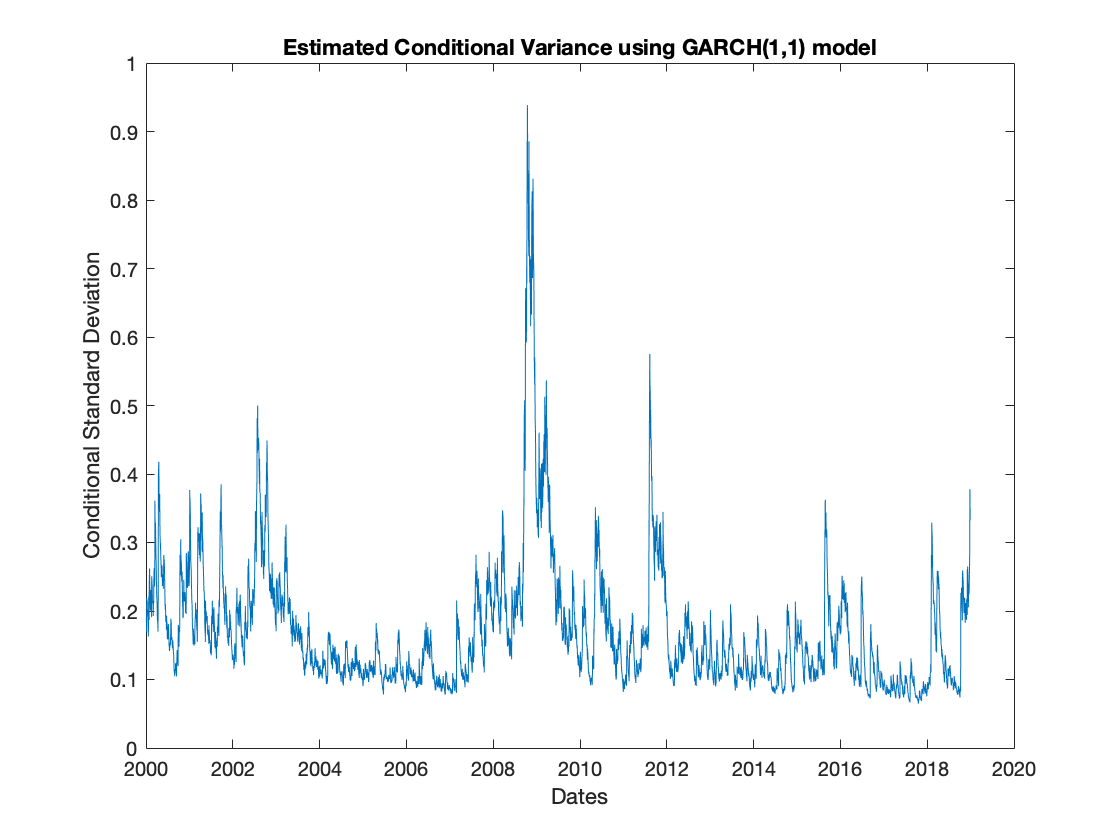
\includegraphics[width = 11cm]{fig/5c}
	\caption{Estimated Conditional Volatility in Annualized Standard Deviation } 
\end{figure}







\end{document}